\documentclass{article}[a4paper]
% Hyperreferences
\usepackage{hyperref}
% Margins
\usepackage[top=35mm,bottom=35mm,left=25mm,right=25mm]{geometry}
% Graphics and images
\usepackage{graphicx} \graphicspath{{./images/}}
\usepackage{subcaption}
\usepackage{float}
% Encodings (to render letters with diacritics and special characters)
\usepackage[utf8]{inputenc}
% Language
\usepackage[english]{babel}
% Section pagebreaks
%\usepackage{titlesec}
%\newcommand{\sectionbreak}{\clearpage}
%\newcommand{\sectionnobreak}{% for when I want a section that does not break
%  \global\toggletrue{afterpart}%
%  \section
%}
% Source code
\usepackage{listings}
\usepackage{xcolor}
\renewcommand{\lstlistingname}{File}
\lstset{
    frame=tb, % draw frame at top and bottom of the code
    tabsize=4, % tab space width
    numbers=left, % display line numbers on the left
	showstringspaces=false, % don't mark spaces in strings    
    commentstyle=\color{green}, % comment color
    keywordstyle=\color{blue}, % keyword color
    stringstyle=\color{red} % string color
}
\lstdefinelanguage{Maxima}{
	keywords={log,jacobian,determinant,subst},
	sensitive=true,
	comment=[n][\itshape]{/*}{*/}
}
% Tables with bold rows
\usepackage{tabularx}
\newcommand\setrow[1]{\gdef\rowmac{#1}#1\ignorespaces}
\newcommand\clearrow{\global\let\rowmac\relax}
\clearrow
\usepackage{multirow}
% Math stuff
\usepackage[mathscr]{euscript}
\usepackage{amsmath,amssymb}
\usepackage{mathtools}
\usepackage{enumitem}
\newcommand{\expnumber}[2]{{#1}\mathrm{e}{#2}} % scientific notation
% Definitions, theorems, remarks,...
\usepackage{amsthm}
\newtheorem{definition}{Definition}[section]
\newtheorem{theorem}{Theorem}[section]
\newtheorem{corollary}{Corollary}[theorem]
\newtheorem{lemma}[theorem]{Lemma}
\renewcommand\qedsymbol{$\blacksquare$}
\theoremstyle{remark}
\newtheorem*{remark}{Remark}
% Contents title
\addto\captionsenglish{\renewcommand*\contentsname{Table of contents}}
% Headers and footers
\usepackage{fancyhdr}
\pagestyle{fancyplain}
\fancyhf{}
\lhead{ \fancyplain{}{Post office management database - Delivery I (BDAD 2019/20)}}
\lfoot{ \fancyplain{}{T6G05}}
\rfoot{ \fancyplain{}{\thepage} }
%
\newcommand{\email}[1]{
{\texttt{\href{mailto:#1}{#1}} }
}
% Metadata
\title{\Huge Post office management database \\ \Large Delivery I \\ \vspace*{4pt} \large BDAD 2019/20}
\author{
T6G05\\
\begin{tabular}{r l}
	\email{up201806429@fe.up.pt} & Diogo Miguel Ferreira Rodrigues        \\
	\email{up201806613@fe.up.pt} & João António Cardoso Vieira e Basto de Sousa \\
	\email{up201806330@fe.up.pt} & Rafael Soares Ribeiro \\
\end{tabular}
}
\date{08/03/2020}
% Document
\begin{document}
\begingroup
	\maketitle
	\let\clearpage\relax
	\setcounter{tocdepth}{3}
	\tableofcontents
\endgroup
\section{Introduction}
This preliminary report further details the project we proposed, evidently showing some minor changes that reflect a more adequate representation of the database required to solve the problem of managing a Post Office, deliberately making little to no reference to the workings of a Postal Service given its complexity would greatly surpass recommendations. \par
A postal service is made up of post offices, where each post office has its own set of employees, vehicles and other attributes. The deliveries each have elements that influence its price as well as the ways they may be delivered and paid for, all of which will be explained more thoroughly through this report.
\section{General classes}
\subsection{ZipCode}
ZIP code, characterized by its number (which is also its principal key), town and country, as well as the postman in charge of distributing mail to postal addresses under that ZIP code.
\subsection{Address}
An address is identified by its unique ID, by the street name, street number, door number, postal code, town and country.
\subsection{PAddress}
A postal address extends an address by also mentioning a person name (addresser or addressee), thus being a subclass of Address. Besides mentioning an origin and destination, a delivery must also mention who the addresser and the addressee are, thus requiring a PAddress instead of an Address.
\section{PostalService}
A postal service has a unique ID, a name and a VAT number, besides having physical locations designated hereinafter post offices, one of them being the headquarters. In this project, a PostalService serves the main purpose of storing the VAT and name of the entity that sells goods to clients, which avoids the need for thorough description of the workings of a PostalService that are not directly handled by a PostOffice.
\subsection{PostOffice}
Post offices are places of contact between the postal service and the clients, where services are provided and purchases take place. A PostOffice is associated with a single PostalService.\par
It is uniquely identified by an ID, and characterized also by its address, a list of employees, and by the assigned vehicles. For this reason, it is directly connected to the classes PostalService, Address, Employee and Vehicle.
\subsection{Vehicle}
A vehicle is used to deliver mail and cannot be assigned to time-overlapping orders, given it can only fulfill an order at a time. It is uniquely identified by its license plate, and for each vehicle we know its capacity, that is, the maximum weight it can carry.
\subsubsection{Motorbike}
A motorbike is a vehicle which can be used to fulfill light orders, thus being a subclass of Vehicle. A light order can otherwise be fulfilled by foot.
\subsubsection{Van}
Like the motorbike, the van extends the class Vehicle, but unlike the motorbike, it can be used to deliver general orders.
\section{Person}
For every person we know the VAT number (also serving as a person ID), name, address, and phone number.
\subsection{Client}
A client is a person which may pay for a good or service via a Bill.
\subsection{Employee}
An employee is a person (thus a subclass of Person) that is employed by the company, which provides him/her with a salary. For every employee we know his base salary.
\subsubsection{Manager}
A manager is an employee who is responsible for monitoring a set of sales employees and postmen.
\subsubsection{ShopKeeper}
A shopKeeper is a sales Employee (thus extending the class Employee) who is responsible for processing sales and registering deliveries that were paid for at the PostOffice or mail collected from post boxes.
\subsubsection{Postman}
A postman is an employee (therefore being a subclass of Employee) responsible for home-to-home mail distribution. A postman is assigned a group of ZIP codes.
\section{Delivery}
A delivery is requested by the client and registered by a shopKeeper. \par
Identifiable by its ID, each delivery keeps track of the time of registration, weight, and the postal addresses of the origin and destination (thus connecting this class to PAddress). A delivery’s price is determined not only by the type of service chosen (Economy, Express or Registered) but also by its category; it is classified as a Document if it weighs under 0.100kg, as Parcel if under 2.000kg or Overweight otherwise.\par
Depending on the delivery, its payment can be done either by the purchase of a stamp (which is only valid should the delivery’s category be Document) and deposit at a postbox, or via a bill.
\subsection{Order}
An order corresponds to a request of transporting a deliverable to its destination.\par
It is characterized by its identification number as well as by the postman assigned to its delivery, by the vehicle used for that end and by the scheduled time of departure from, and arrival to, the post office by the postman.\par
It can either be a General Order or a Light Order depending on the category (and therefore on the weight) of the deliverables: light orders can only be used for deliveries which have Documents as its category.
\subsection{Stamp}
A stamp is an alternative to paying for a Document using a bill. A stamped document can be deposited in a postbox. Given stamps are specialized according to the service that will be used in transporting the Document, Stamp is associated to the class Service.
\subsection{Bill}
A bill can be used to buy products at a PostOffice, as well as to pay for any kind of deliverable. A bill is described by its bill number, price (which is the sum of prices of the items of the delivery), issue time, issuing shopKeeper, the client that paid for it and the seller, which is the company to which the client is paying for a delivery.
\subsection{Product}
Each product has a corresponding ID (similar to a barcode), description and current price. The list of all products make up the catalog of products the PostalService has for sale.
\subsection{Item}
An item is a particular instance of a product, for which a client paid a given sum. It is identifiable by its ID (similar to a serial number) and by its price at the moment it was bought.
\section{UML}
\begin{figure}[H] \centering
	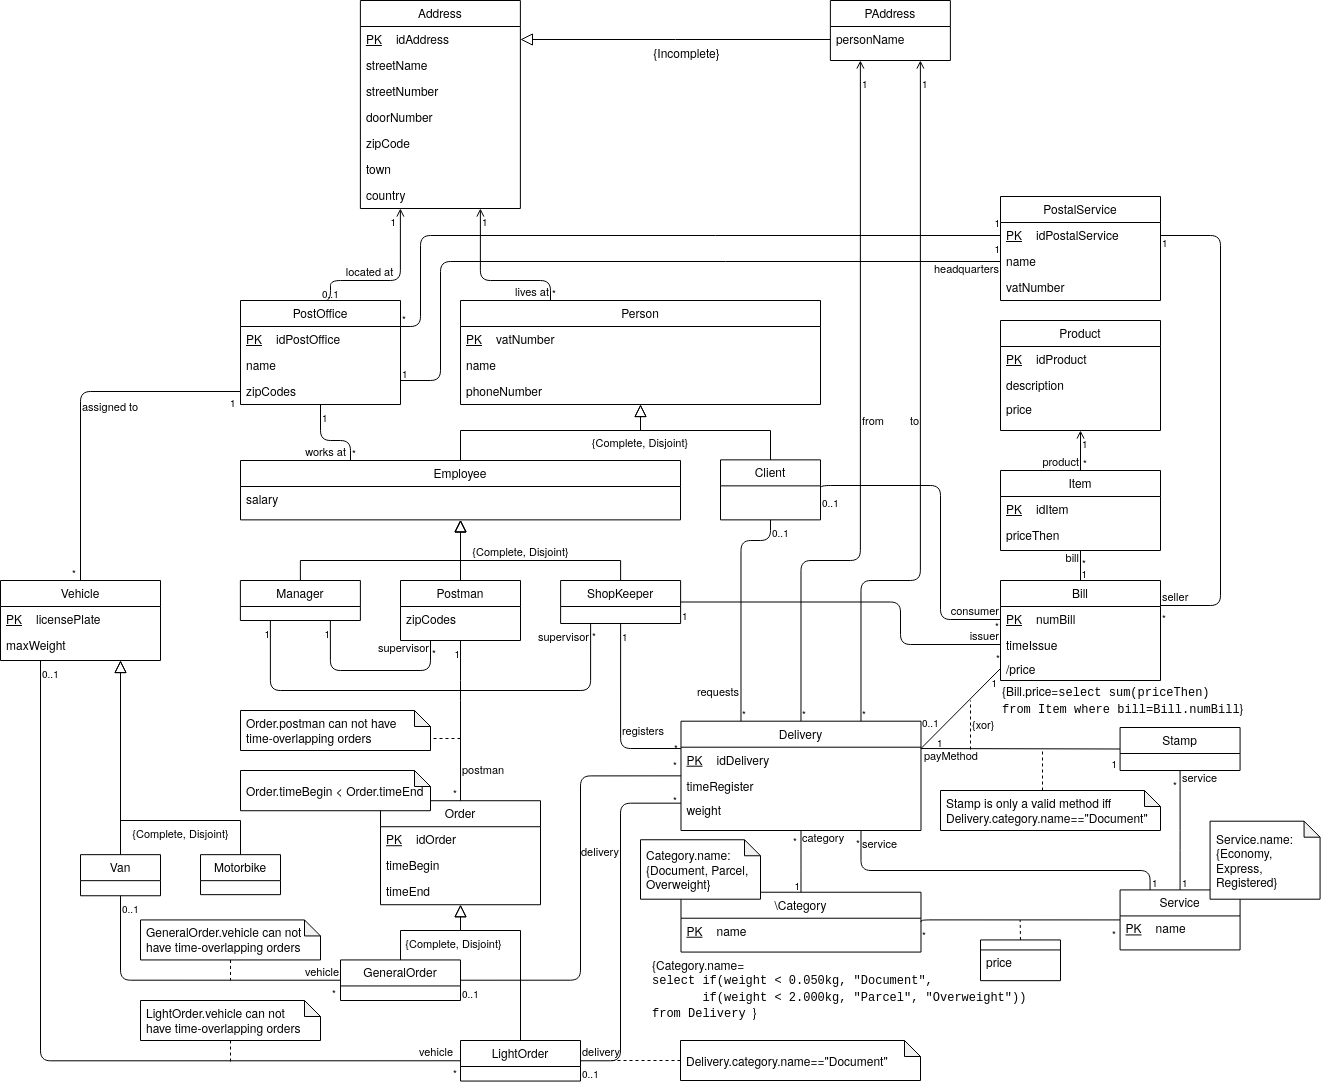
\includegraphics[angle=-90,scale=0.397]{uml}
	\caption{Database UML}
\end{figure}
\end{document}
